% DotCompute Executive Overview
% Compile with: pdflatex dotcompute-executive-overview.tex (run twice for TOC)
\documentclass[11pt,a4paper]{article}

% ── Packages ──────────────────────────────────────────────────────────────────
\usepackage[utf8]{inputenc}
\usepackage[T1]{fontenc}
\usepackage{lmodern}
\usepackage[margin=2.4cm]{geometry}
\usepackage{graphicx}
\usepackage{xcolor}
\usepackage{titlesec}
\usepackage{enumitem}
\usepackage{booktabs}
\usepackage{tabularx}
\usepackage{colortbl}
\usepackage{multirow}
\usepackage{fancyhdr}
\usepackage{hyperref}
\usepackage{amssymb}
\usepackage{tcolorbox}
\usepackage{tikz}
\usetikzlibrary{arrows.meta, positioning, calc, shapes.geometric, backgrounds, fit}

% ── Colours ───────────────────────────────────────────────────────────────────
\definecolor{brand}{HTML}{1A2744}      % Deep navy
\definecolor{accent}{HTML}{E8700A}     % Burnt orange
\definecolor{highlight}{HTML}{F5A623}  % Amber gold
\definecolor{success}{HTML}{2D936C}    % Green
\definecolor{lightbg}{HTML}{F5F7FA}    % Light background
\definecolor{midgray}{HTML}{6C757D}    % Muted text

% ── Heading styles ────────────────────────────────────────────────────────────
\titleformat{\section}
  {\Large\bfseries\color{brand}}
  {\thesection}{1em}{}[\vspace{-0.4em}\textcolor{accent}{\rule{\textwidth}{1.2pt}}]

\titleformat{\subsection}
  {\large\bfseries\color{brand}}
  {\thesubsection}{0.8em}{}

\titleformat{\subsubsection}
  {\normalsize\bfseries\color{accent}}
  {\thesubsubsection}{0.6em}{}

% ── Header / Footer ──────────────────────────────────────────────────────────
\pagestyle{fancy}
\fancyhf{}
\renewcommand{\headrulewidth}{0.4pt}
\fancyhead[L]{\small\textcolor{midgray}{DotCompute --- Executive Overview}}
\fancyhead[R]{\small\textcolor{midgray}{v0.5.3}}
\fancyfoot[C]{\small\textcolor{midgray}{\thepage}}

% ── Custom boxes ──────────────────────────────────────────────────────────────
\tcbset{
  keybox/.style={
    colback=lightbg, colframe=accent, boxrule=0.6pt,
    arc=3pt, left=8pt, right=8pt, top=6pt, bottom=6pt,
    colbacktitle=accent, coltitle=white,
    fonttitle=\bfseries, title=#1
  },
  statbox/.style={
    colback=white, colframe=brand, boxrule=0.8pt,
    arc=4pt, left=6pt, right=6pt, top=4pt, bottom=4pt,
    width=0.30\textwidth
  }
}

% ── Hyperref setup ────────────────────────────────────────────────────────────
\hypersetup{
  colorlinks=true,
  linkcolor=brand,
  urlcolor=accent,
  citecolor=brand,
  pdftitle={DotCompute -- GPU Acceleration Framework for .NET},
  pdfauthor={Michael Ivertowski},
  pdfsubject={Executive Overview},
}

% ══════════════════════════════════════════════════════════════════════════════
\begin{document}

% ── Title page ────────────────────────────────────────────────────────────────
\begin{titlepage}
\begin{tikzpicture}[remember picture, overlay]
  % Background gradient bar
  \fill[brand] (current page.north west) rectangle
    ([yshift=-9cm]current page.north east);
  % Accent stripe
  \fill[accent] ([yshift=-9cm]current page.north west) rectangle
    ([yshift=-9.4cm]current page.north east);
  % Decorative dots
  \foreach \x in {0.5,1.0,...,5.0} {
    \foreach \y in {0.5,1.0,...,3.0} {
      \fill[white, opacity=0.04] ([xshift=\x cm, yshift=-\y cm]current page.north west)
        circle (1.5pt);
    }
  }
\end{tikzpicture}

\vspace*{1.5cm}
\begin{flushleft}
  {\fontsize{38}{44}\selectfont\bfseries\textcolor{white}{DotCompute}}\\[0.5em]
  {\fontsize{16}{20}\selectfont\textcolor{white!85}{GPU Acceleration Framework for .NET}}\\[0.3em]
  {\large\textcolor{white!65}{High-Performance SIMD, CUDA, OpenCL \& Metal Compute}}\\[0.3em]
  {\normalsize\textcolor{white!50}{.NET 9 \textbullet{} Native AOT \textbullet{} Source Generators \textbullet{} Roslyn Analyzers}}
\end{flushleft}

\vspace{5.5cm}

\begin{flushleft}
  \textcolor{midgray}{\large Executive Overview}\\[0.8em]
  {\Large\textcolor{brand}{\textbf{Version 0.5.3}}}\\[1.5em]
  \textcolor{midgray}{%
    A production-grade .NET GPU acceleration framework delivering\\
    CPU 3.7x (SIMD) and GPU 21--92x (CUDA) speedups with\\
    native AOT support, source generators, and multi-backend compute.%
  }
\end{flushleft}

\vfill
\begin{flushleft}
  \textcolor{midgray}{\small
    Built with C\# 13 \& .NET 9 \textbullet{} 4-layer architecture \textbullet{} 5 compute backends\\[4pt]
    Open-source (MIT License) \textbullet{} NuGet packages available\\[4pt]
    \textbf{Repository:} \href{https://github.com/mivertowski/DotCompute}{github.com/mivertowski/DotCompute}\\[4pt]
    \textbf{Documentation:} \href{https://mivertowski.github.io/DotCompute/}{mivertowski.github.io/DotCompute}\\[4pt]
    \textbf{Contact:} \href{mailto:michael.ivertowski@ch.ey.com}{michael.ivertowski@ch.ey.com}
  }
\end{flushleft}
\end{titlepage}

% ── Table of Contents ─────────────────────────────────────────────────────────
\tableofcontents
\newpage

% ══════════════════════════════════════════════════════════════════════════════
\section{Executive Summary}

DotCompute is a production-grade GPU acceleration framework for .NET~9+,
designed to bring high-performance parallel computing to the .NET ecosystem.
It provides a unified programming model across CPU (AVX2/AVX512/NEON SIMD),
CUDA, OpenCL, and Metal backends --- enabling developers to write compute
kernels once and execute them on any supported hardware with automatic
backend selection and optimization.

\begin{tcolorbox}[keybox={Why DotCompute?}]
\begin{itemize}[leftmargin=1.2em, itemsep=3pt]
  \item \textbf{Massive speedups} --- CPU SIMD delivers 3.7x, CUDA delivers
        21--92x over baseline on NVIDIA RTX hardware (Compute Capability~8.9).
  \item \textbf{Native AOT compatible} --- sub-10\,ms startup with no runtime
        code generation; source generators handle all compile-time codegen.
  \item \textbf{Multi-backend compute} --- write once, run on CPU, CUDA,
        OpenCL, or Metal with automatic backend selection.
  \item \textbf{Developer tooling} --- 12 Roslyn diagnostic rules, 5 automated
        code fixes, and \texttt{[Kernel]} attribute-driven source generation
        provide real-time IDE feedback.
  \item \textbf{Production infrastructure} --- memory pooling (90\%
        allocation reduction), P2P transfers, dependency injection integration,
        and plugin system with hot-reload capability.
\end{itemize}
\end{tcolorbox}

\subsection{At a Glance}

\vspace{0.6em}
\begin{center}
\begin{tabular}{@{}c@{\hspace{1.8em}}c@{\hspace{1.8em}}c@{}}
\begin{tcolorbox}[statbox, width=4.8cm]
  \centering
  {\fontsize{26}{30}\selectfont\bfseries\textcolor{accent}{92x}}\\[3pt]
  {\small peak GPU speedup (CUDA)}
\end{tcolorbox} &
\begin{tcolorbox}[statbox, width=4.8cm]
  \centering
  {\fontsize{26}{30}\selectfont\bfseries\textcolor{accent}{5}}\\[3pt]
  {\small compute backends}
\end{tcolorbox} &
\begin{tcolorbox}[statbox, width=4.8cm]
  \centering
  {\fontsize{26}{30}\selectfont\bfseries\textcolor{accent}{$<$10\,ms}}\\[3pt]
  {\small Native AOT startup}
\end{tcolorbox}
\end{tabular}
\end{center}

% ══════════════════════════════════════════════════════════════════════════════
\newpage
\section{Compute Backends}

DotCompute provides five compute backends, each optimized for specific
hardware targets while sharing a unified kernel programming model.

\noindent
\renewcommand{\arraystretch}{1.25}
\begin{tabularx}{\textwidth}{>{\bfseries\color{brand}}l c c X}
\toprule
\rowcolor{accent} \textcolor{white}{\textbf{Backend}} & \textcolor{white}{\textbf{Status}} & \textcolor{white}{\textbf{Speedup}} & \textcolor{white}{\textbf{Capabilities}} \\
\midrule
CPU &
  Production & 3.7x &
  AVX2, AVX512, and ARM NEON SIMD intrinsics;
  thread-based persistent kernel execution. \\
CUDA &
  Production & 21--92x &
  Compute Capability 5.0--8.9; CUBIN (CC $\geq$ 7.0) and PTX compilation;
  P2P transfers; NCCL multi-GPU; Ring Kernels. \\
OpenCL &
  Experimental & --- &
  Cross-platform support for NVIDIA, AMD, Intel, ARM Mali, and Qualcomm
  Adreno GPUs. \\
Metal &
  Feature-Complete & --- &
  Apple GPU via Metal Performance Shaders; MSL kernel translation;
  Ring Kernel execution; memory pooling. \\
ROCm &
  Placeholder & --- &
  AMD GPU backend planned for future development. \\
\bottomrule
\end{tabularx}

\noindent
An \textbf{Adaptive Backend Selector} uses ML-powered heuristics to
automatically choose the optimal backend based on data size, kernel
complexity, hardware availability, and historical profiling data.

% ══════════════════════════════════════════════════════════════════════════════
\section{Kernel Programming Model}

DotCompute provides a modern, attribute-driven kernel programming model
that eliminates boilerplate and enables compile-time optimization through
source generators.

\subsection{Kernel Authoring}

\begin{tcolorbox}[colback=brand!3, colframe=brand!40, boxrule=0.5pt, arc=3pt,
                   left=8pt, right=8pt, top=6pt, bottom=6pt]
\ttfamily\small
[Kernel]\\
public static void VectorAdd(\\
\hspace{2em}ReadOnlySpan<float> a,\\
\hspace{2em}ReadOnlySpan<float> b,\\
\hspace{2em}Span<float> result)\\
\{\\
\hspace{2em}int idx = Kernel.ThreadId.X;\\
\hspace{2em}if (idx < result.Length)\\
\hspace{4em}result[idx] = a[idx] + b[idx];\\
\}
\end{tcolorbox}

\noindent
The \texttt{[Kernel]} attribute triggers source generation at compile time,
producing optimized wrappers for each target backend. No runtime reflection
or code generation is required, preserving full Native AOT compatibility.
The pipeline is: \texttt{C\# Source} $\to$ \texttt{Roslyn Analysis} (12 rules)
$\to$ \texttt{Source Generation} $\to$ \texttt{Backend Wrappers}.

\subsection{Kernel System Components}

\noindent
\renewcommand{\arraystretch}{1.2}
\begin{tabularx}{\textwidth}{>{\bfseries\color{brand}}l X}
\toprule
\rowcolor{accent} \textcolor{white}{\textbf{Component}} & \textcolor{white}{\textbf{Description}} \\
\midrule
IKernelCompiler &
  Backend-specific kernel compilation (PTX, SPIR-V, MSL, SIMD). \\
KernelDefinition &
  Metadata describing kernel signature, thread dimensions, and
  compilation options. \\
ICompiledKernel &
  Ready-to-execute kernel with launch configuration and resource bindings. \\
CompilationOptions &
  Optimization level, debug info, target compute capability, and
  backend-specific flags. \\
\bottomrule
\end{tabularx}

\subsection{Roslyn Analyzers (DC001--DC012)}

\noindent
\renewcommand{\arraystretch}{1.2}
\begin{tabularx}{\textwidth}{>{\bfseries\color{brand}}l l X}
\toprule
\rowcolor{accent} \textcolor{white}{\textbf{Rule}} & \textcolor{white}{\textbf{Severity}} & \textcolor{white}{\textbf{Description}} \\
\midrule
DC001--DC004 & Error    & Kernel signature validation (return type, parameters, static) \\
DC005--DC008 & Warning  & Memory access patterns and bounds checking \\
DC009--DC010 & Warning  & Thread divergence and synchronization issues \\
DC011--DC012 & Info     & Performance hints and optimization suggestions \\
\bottomrule
\end{tabularx}

\vspace{0.5em}
\noindent
All rules include \textbf{5 automated code fixes} for one-click resolution
of common kernel authoring issues directly in the IDE.

% ══════════════════════════════════════════════════════════════════════════════
\section{Ring Kernel System}

The Ring Kernel system implements a persistent GPU computation model based
on the actor pattern, enabling long-lived GPU kernels that process messages
with sub-microsecond serialization. The pipeline flows from host application
through a message bridge and MemoryPack serialization ($<$100\,ns) to a
persistent or event-driven GPU kernel.

\subsection{Implementation Phases}

\noindent
\renewcommand{\arraystretch}{1.25}
\begin{tabularx}{\textwidth}{>{\bfseries\color{brand}}l c X}
\toprule
\rowcolor{accent} \textcolor{white}{\textbf{Phase}} & \textcolor{white}{\textbf{Status}} & \textcolor{white}{\textbf{Capabilities}} \\
\midrule
Phase 1: MemoryPack &
  Complete &
  Auto-discovery of \texttt{[MemoryPackable]} types via Roslyn; batch CUDA
  codegen for 10+ message types; $<$100\,ns serialization. \\
Phase 2: CPU Ring &
  Complete &
  Thread-based persistent kernels; message queue bridge; echo mode with
  intelligent transformation; full lifecycle management. \\
Phase 3: CUDA Ring &
  94.3\% &
  End-to-end GPU message processing; 6-stage compilation pipeline;
  $\sim$1.24\,$\mu$s serialization. \\
Phase 4: Multi-GPU &
  Complete &
  P2P memory transfer infrastructure; cross-GPU barrier foundations;
  coordination primitives for multi-device setups. \\
Phase 5: Observability &
  Complete &
  OpenTelemetry integration; Prometheus-compatible metrics; health checks;
  fault tolerance with Polly resilience policies. \\
\bottomrule
\end{tabularx}

\subsection{GPU Compute Primitives}

\noindent
\renewcommand{\arraystretch}{1.2}
\begin{tabularx}{\textwidth}{>{\bfseries\color{brand}}l X}
\toprule
\rowcolor{accent} \textcolor{white}{\textbf{API}} & \textcolor{white}{\textbf{Details}} \\
\midrule
GPU Timing &
  1\,ns resolution on CC~6.0+, 4 calibration strategies, per-kernel profiling. \\
Barrier API &
  ThreadBlock, Grid, Warp, and Named barriers with $<$20\,ns overhead. \\
Memory Ordering &
  3 consistency models (relaxed, acquire-release, sequential) with
  proper fence semantics. \\
Unified Buffer &
  Cross-device memory abstraction with automatic transfer management
  and pooled allocation. \\
\bottomrule
\end{tabularx}

% ══════════════════════════════════════════════════════════════════════════════
\section{Memory Management}

DotCompute provides a layered memory subsystem that minimizes allocation
overhead and automates cross-device transfers:

\begin{itemize}[leftmargin=1.4em, itemsep=2pt]
  \item \textbf{UnifiedBuffer<T>}: Generic, type-safe buffer abstraction
        that works identically across CPU, CUDA, OpenCL, and Metal with
        automatic lifecycle management.
  \item \textbf{Memory pooling}: Size-class bucketed allocation pool
        reduces GC pressure and achieves 90\% fewer allocations.
  \item \textbf{Automatic transfers}: The runtime transparently moves data
        between host (pinned) and device (VRAM) as kernels require.
  \item \textbf{P2P transfers}: Direct GPU-to-GPU copies for multi-device
        workloads without host memory round-trips.
  \item \textbf{Bounds validation}: Debug-mode bounds checking in kernels
        catches out-of-range accesses before they corrupt memory.
\end{itemize}

% ══════════════════════════════════════════════════════════════════════════════
\section{Developer Tooling \& Runtime}

DotCompute integrates deeply into the .NET developer workflow through
source generators, Roslyn analyzers, and runtime infrastructure.

\noindent
\renewcommand{\arraystretch}{1.2}
\begin{tabularx}{\textwidth}{>{\bfseries\color{brand}}l X}
\toprule
\rowcolor{accent} \textcolor{white}{\textbf{Component}} & \textcolor{white}{\textbf{Description}} \\
\midrule
Source Generators &
  Roslyn-based compile-time codegen from \texttt{[Kernel]} attributes;
  produces backend-specific wrappers with zero runtime reflection. \\
DI Integration &
  Full Microsoft.Extensions.DependencyInjection support with
  \texttt{AddDotCompute()} service registration. \\
Plugin System &
  Hot-reload capable plugin architecture for custom backends
  and kernel providers. \\
Orchestrator &
  \texttt{IComputeOrchestrator} manages kernel compilation, execution,
  and resource lifecycle. \\
Debug Service &
  \texttt{IKernelDebugService} enables CPU vs.\ GPU result validation
  for cross-backend debugging. \\
Adaptive Optimizer &
  ML-powered \texttt{AdaptiveBackendSelector} learns optimal backend
  assignments from runtime profiling. \\
\bottomrule
\end{tabularx}

% ══════════════════════════════════════════════════════════════════════════════
\section{LINQ Extensions}

DotCompute extends .NET LINQ with GPU-accelerated query execution,
enabling familiar \texttt{Select}, \texttt{Where}, and \texttt{Aggregate}
operations to transparently compile to GPU kernels. Adjacent operations
are automatically fused into single kernel launches to reduce overhead.

\noindent
\renewcommand{\arraystretch}{1.2}
\begin{tabularx}{\textwidth}{>{\bfseries\color{brand}}l c X}
\toprule
\rowcolor{accent} \textcolor{white}{\textbf{Operation}} & \textcolor{white}{\textbf{Status}} & \textcolor{white}{\textbf{Details}} \\
\midrule
Select / Map      & Complete & Element-wise transformations with GPU codegen. \\
Where / Filter    & Complete & Predicate evaluation with stream compaction. \\
Aggregate / Reduce & Complete & Parallel reduction with configurable operators. \\
Kernel Fusion     & Complete & Adjacent operations merged into single kernel launch. \\
Join              & Planned & Hash-based GPU join for relational operations. \\
GroupBy           & Planned & GPU-accelerated grouping with aggregation. \\
OrderBy           & Planned & Parallel sort (bitonic/radix) on GPU. \\
\bottomrule
\end{tabularx}

% ══════════════════════════════════════════════════════════════════════════════
\section{Architecture}

\begin{center}
\resizebox{\textwidth}{!}{%
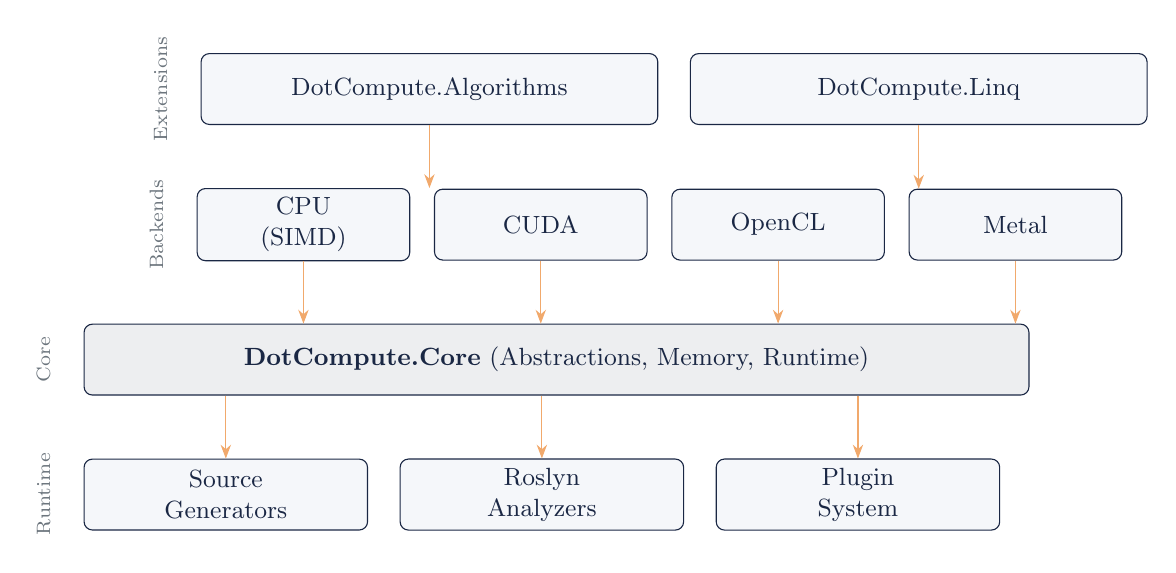
\begin{tikzpicture}[
  node distance=0.5cm,
  layer/.style={draw=brand, fill=lightbg, rounded corners=3pt,
                minimum height=0.9cm, font=\small, text=brand, align=center},
  arr/.style={-{Stealth[length=5pt]}, color=accent!60}
]
  % Extensions layer
  \node[layer, minimum width=5.8cm] (algo) {DotCompute.Algorithms};
  \node[layer, minimum width=5.8cm, right=0.4cm of algo] (linq) {DotCompute.Linq};

  % Label
  \node[left=0.3cm of algo, font=\scriptsize\color{midgray}, rotate=90, anchor=south]
    {Extensions};

  % Backends layer
  \node[layer, minimum width=2.7cm, below=0.8cm of algo, anchor=north, xshift=-1.6cm]
    (cpu) {CPU\\(SIMD)};
  \node[layer, minimum width=2.7cm, right=0.3cm of cpu]
    (cuda) {CUDA};
  \node[layer, minimum width=2.7cm, right=0.3cm of cuda]
    (opencl) {OpenCL};
  \node[layer, minimum width=2.7cm, right=0.3cm of opencl]
    (metal) {Metal};

  \node[left=0.3cm of cpu, font=\scriptsize\color{midgray}, rotate=90, anchor=south]
    {Backends};

  % Core layer
  \node[layer, minimum width=12cm, below=0.8cm of cuda, anchor=north,
        xshift=0.2cm, fill=brand!8]
    (core) {\textbf{DotCompute.Core} (Abstractions, Memory, Runtime)};

  \node[left=0.3cm of core, font=\scriptsize\color{midgray}, rotate=90, anchor=south]
    {Core};

  % Runtime layer
  \node[layer, minimum width=3.6cm, below=0.8cm of core, xshift=-4.2cm]
    (generators) {Source\\Generators};
  \node[layer, minimum width=3.6cm, right=0.4cm of generators]
    (analyzers) {Roslyn\\Analyzers};
  \node[layer, minimum width=3.6cm, right=0.4cm of analyzers]
    (plugins) {Plugin\\System};

  \node[left=0.3cm of generators, font=\scriptsize\color{midgray}, rotate=90, anchor=south]
    {Runtime};

  % Arrows
  \draw[arr] (algo.south) -- (algo.south |- cpu.north);
  \draw[arr] (linq.south) -- (linq.south |- opencl.north);

  \draw[arr] (cpu.south) -- (cpu.south |- core.north);
  \draw[arr] (cuda.south) -- (cuda.south |- core.north);
  \draw[arr] (opencl.south) -- (opencl.south |- core.north);
  \draw[arr] (metal.south) -- (metal.south |- core.north);

  \draw[arr] (core.south -| generators) -- (generators.north);
  \draw[arr] (core.south -| analyzers) -- (analyzers.north);
  \draw[arr] (core.south -| plugins) -- (plugins.north);
\end{tikzpicture}%
}% end resizebox
\end{center}

% ══════════════════════════════════════════════════════════════════════════════
\section{Use Cases}

\begin{tcolorbox}[keybox={Primary Use Cases}]
\begin{description}[leftmargin=1em, labelwidth=1em, font=\color{brand}\bfseries]
  \item[$\blacktriangleright$] \textbf{Scientific Computing} ---
    GPU-accelerated linear algebra, matrix operations, and numerical
    simulations with 21--92x speedups on NVIDIA hardware.

  \item[$\blacktriangleright$] \textbf{Machine Learning Inference} ---
    High-throughput tensor operations for .NET ML pipelines with
    automatic SIMD/CUDA backend selection.

  \item[$\blacktriangleright$] \textbf{Data Processing Pipelines} ---
    GPU-accelerated LINQ extensions for large-scale data transformations
    with kernel fusion optimization.

  \item[$\blacktriangleright$] \textbf{Real-Time Signal Processing} ---
    Ring Kernel actor model for persistent GPU computation with
    sub-microsecond message serialization.

  \item[$\blacktriangleright$] \textbf{Financial Computing} ---
    Monte Carlo simulations, risk calculations, and portfolio optimization
    leveraging GPU parallelism.

  \item[$\blacktriangleright$] \textbf{Cross-Platform GPU Compute} ---
    Write-once kernels targeting Windows (CUDA/OpenCL), macOS (Metal),
    and Linux (CUDA/OpenCL) from a single .NET codebase.
\end{description}
\end{tcolorbox}

% ══════════════════════════════════════════════════════════════════════════════
\section{Getting Started}

\subsection{Installation}

\begin{tcolorbox}[colback=brand!3, colframe=brand!40, boxrule=0.5pt, arc=3pt,
                   left=8pt, right=8pt, top=6pt, bottom=6pt]
\ttfamily\small
\# Add DotCompute NuGet packages\\
dotnet add package DotCompute.Core\\
dotnet add package DotCompute.Backend.Cpu\\
dotnet add package DotCompute.Backend.Cuda \hspace{1em}\# NVIDIA GPU\\
dotnet add package DotCompute.Backend.Metal \hspace{0.5em}\# Apple GPU
\end{tcolorbox}

\subsection{Quick Start}

\begin{tcolorbox}[colback=brand!3, colframe=brand!40, boxrule=0.5pt, arc=3pt,
                   left=8pt, right=8pt, top=6pt, bottom=6pt]
\ttfamily\small
\# Build the solution\\
dotnet build DotCompute.sln --configuration Release\\[6pt]
\# Run all tests (recommended --- auto-configures WSL2)\\
./scripts/run-tests.sh DotCompute.sln --configuration Release\\[6pt]
\# Run specific test categories\\
./scripts/run-tests.sh DotCompute.sln --filter "Category=Unit"\\
./scripts/run-tests.sh DotCompute.sln --filter "Category=Hardware"
\end{tcolorbox}

\subsection{Requirements}

\begin{itemize}[leftmargin=1.4em, itemsep=2pt]
  \item .NET 9.0 SDK or later (C\# 13 language features)
  \item Visual Studio 2022 17.8+ or VS Code with C\# Dev Kit
  \item CUDA Toolkit 12.0+ (for GPU support)
  \item NVIDIA GPU with Compute Capability 5.0+ (for CUDA tests)
\end{itemize}

% ══════════════════════════════════════════════════════════════════════════════
\vspace{1.5em}
\begin{tcolorbox}[keybox={Links \& Resources}]
\renewcommand{\arraystretch}{1.4}
\begin{tabularx}{\textwidth}{>{\bfseries\color{brand}}l X}
  Repository &
    \url{https://github.com/mivertowski/DotCompute} \\
  Documentation &
    \url{https://mivertowski.github.io/DotCompute/} \\
  NuGet &
    DotCompute.Core, DotCompute.Backend.Cpu, DotCompute.Backend.Cuda \\
\end{tabularx}
\end{tcolorbox}

\vfill
\begin{center}
\textcolor{midgray}{\rule{0.5\textwidth}{0.4pt}}\\[0.8em]
{\small\textcolor{midgray}{%
  DotCompute v0.5.3 \textbullet{}
  MIT License \textbullet{}
  .NET 9+ \textbullet{}
  Native AOT Compatible%
}}\\[4pt]
{\small\textcolor{midgray}{%
  \textbf{Contact:} \href{mailto:michael.ivertowski@ch.ey.com}{michael.ivertowski@ch.ey.com}%
}}
\end{center}

\end{document}
